\chapter{Model Matematyczny}
\label{cha:math_model}

\section{Noga robota typu RRR}

Noga ma trzy stopnie swobody. Wszystkie są typu obrotowego, co czyni z niej konstrukcję typu $RRR$. Przy czym dwa elementy rotacyjne obracają się dookoła osi poziomej ($X$) (podobnie jak w przypadku robota STriDER), a jedna dookoła osi pionowej ($Z$). Są to też te same osi obrotu co w przypadku ramienia robotycznego typu antromorficznego (zwanego także "angular" bądź "jointed"). Co za tym idzie, cały model matematyczny jest w zasadzie identyczny jak w przypadku manipulatora tego typu.\\

\begin{figure}[h!]
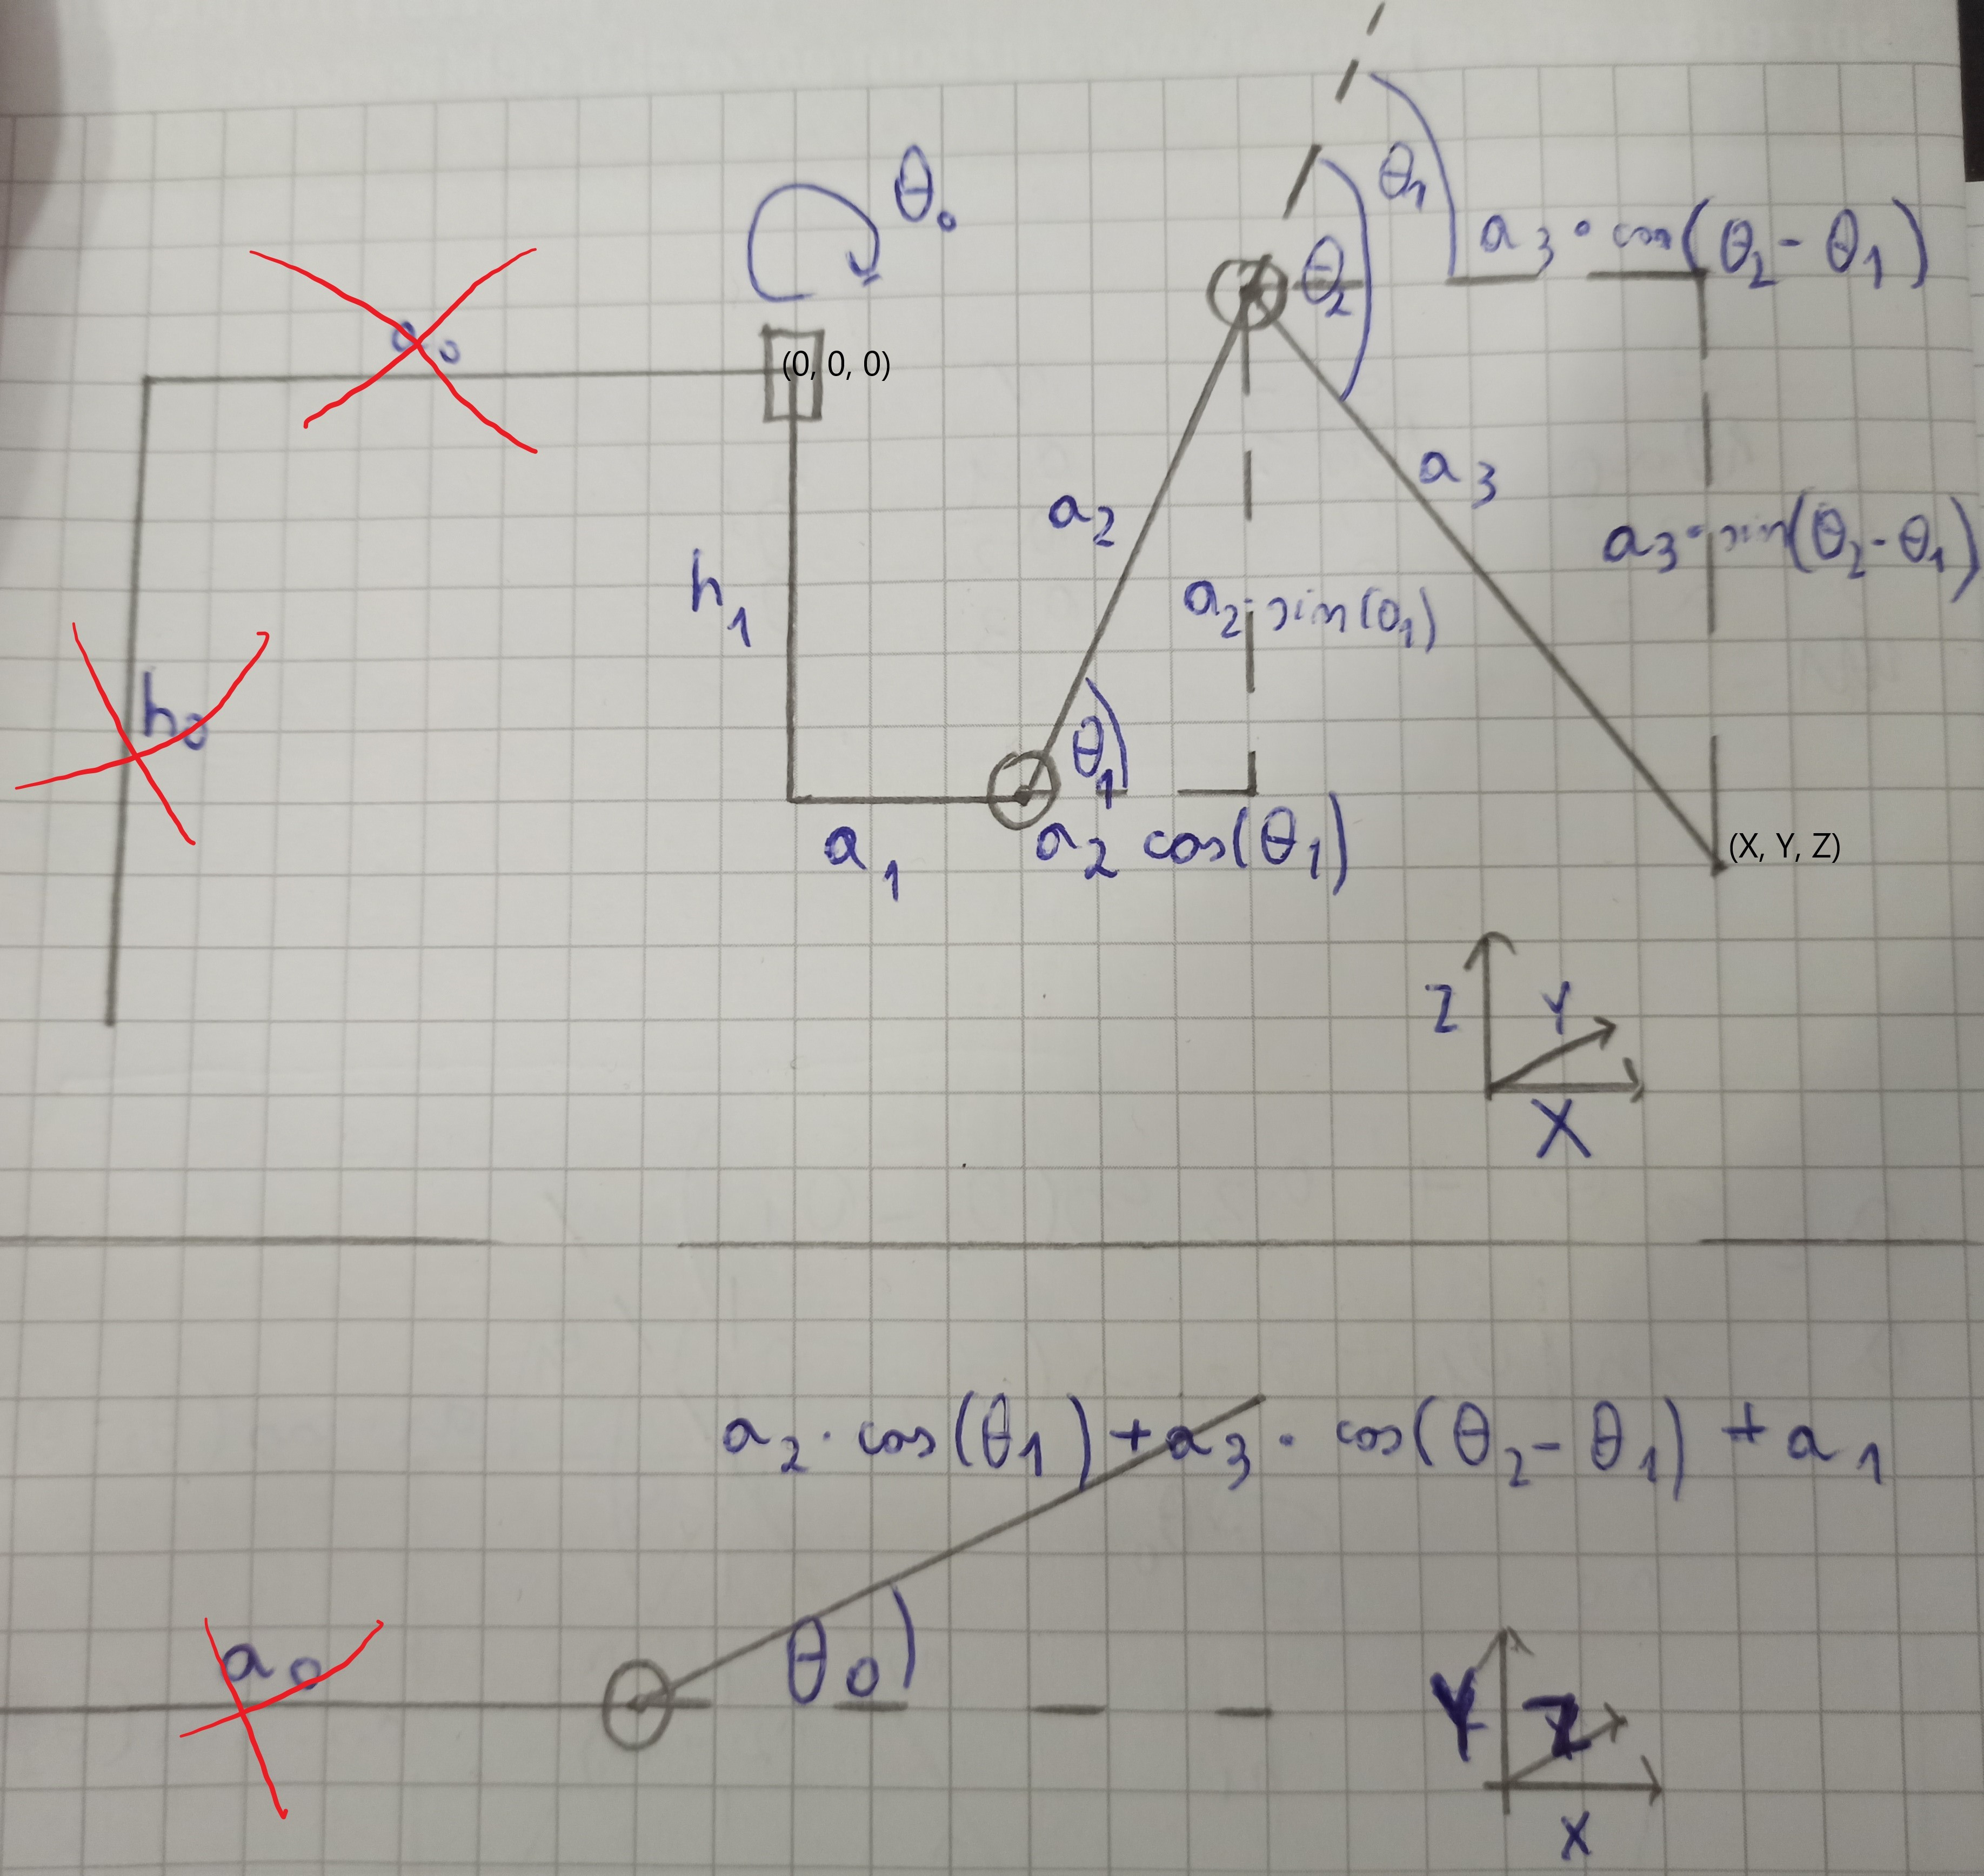
\includegraphics[width=\textwidth]{img/math_model.jpg}
\caption{Model Matematyczny}
\label{math_model}
\end{figure}

\subsection{Kinematyka Prosta}
Obliczanie kinematyki prostej polega na uzyskniu równań końcówki ramienia robotycznego we współrzędnych kartezjańskich względem współrzędnych konfiguracyjnych. Inaczej mówiąc, wejściem algorytmu jest zbiór współrzędnych konfiguracyjnych, a na wyjściu otrzymamy współrzędne kartezjańskie.\cite{robot_manipulators}\\

W przypadku tego konkretnego manipulatora, mamy do czynienia z trójwymiarowym układem współrzędnych kartezjańskich i trzema stopniami swobody. Da to liniowo niezależny układ trzech równań, w którym parametrami będą kąty na jakich mają ustawić się serwomechanizmy a wynikiem wektor współrzędnych kartezjańskich.\\

Najprostszą metodą liczenia kinematyki prostej jest rozrysowanie modelu matematycznego i geometryczne wyprowadzenie potrzebnych równań. Model taki dla tego manipulatora został przedstawiony na rysunku \ref{math_model}. Przyjęty początek układu współrzędnych został oznaczony jako $(0, 0, 0)$, a punkt którego współrzędne kartezjańskie są poszukiwane został oznaczony jako $(X, Y, Z)$. $h_1$ i $a_{1-3}$ to stałe długości poszczególnych członów nogi. Natomiast $\theta_{0-2}$ to właśnie pozycje serwomechanizmów - parametry algorytmu. Na ich podstawie zostaną obliczone współrzędne końcówki manipulatora w systemie kartezjańskim. Same obliczenia geometryczne są już w tym momencie dość trywialne, wystarczy do każdego członu $a_{1-3}$ przenieść jego długość na oś $X$, $Y$ lub $Z$ za pomocą trygonometrii (sinus lub cosinus) i zsumować odpowiednie długości. Da to układ równań \ref{FK_ver_1}.\\

\begin{equation} \label{FK_ver_1}
\begin{split}
a_{temp} &= a_2 \cos{\theta_1} + a_3 \cos{\left(\theta_2 - \theta_1\right)} + a_1\\
Y &= a_{temp} \cdot \sin{\theta_0}\\
X &= a_{temp} \cdot \cos{\theta_0}\\
Z &= a_2 \sin{\theta_1} - a_3 \sin{\left(\theta_2 - \theta_1\right)}
\end{split}
\end{equation}

\subsection{Kinematyka prosta - metoda Denavita Hartenberga \cite{DH_AA_article}}
Alternatywą dla zwykłych obliczeń geometrycznych jest metoda Denvaita Hartenberga. Polega ona na przedstawieniu całkowitego przekształcenia jako iloczynu przekształceń jednorodnych kolejnych członów. Pojedyncze przekształcenie jednorodne składa się natomiast z 6 przekształceń prostych (3 dla rotacji i 3 dla przesunięć). Wymnożenie tych przekształceń prostych da przekształcenie jednorodne. \cite{DH_wpaszke_wyklad}\\

Metoda ta jest w szczególności użyteczna dla bardzo skomplikowanych manipulatorów, gdzie stopni swobody jest znacznie więcej niż ilość współrzędnych kartezjańskich.\\

\begin{figure}[h!]
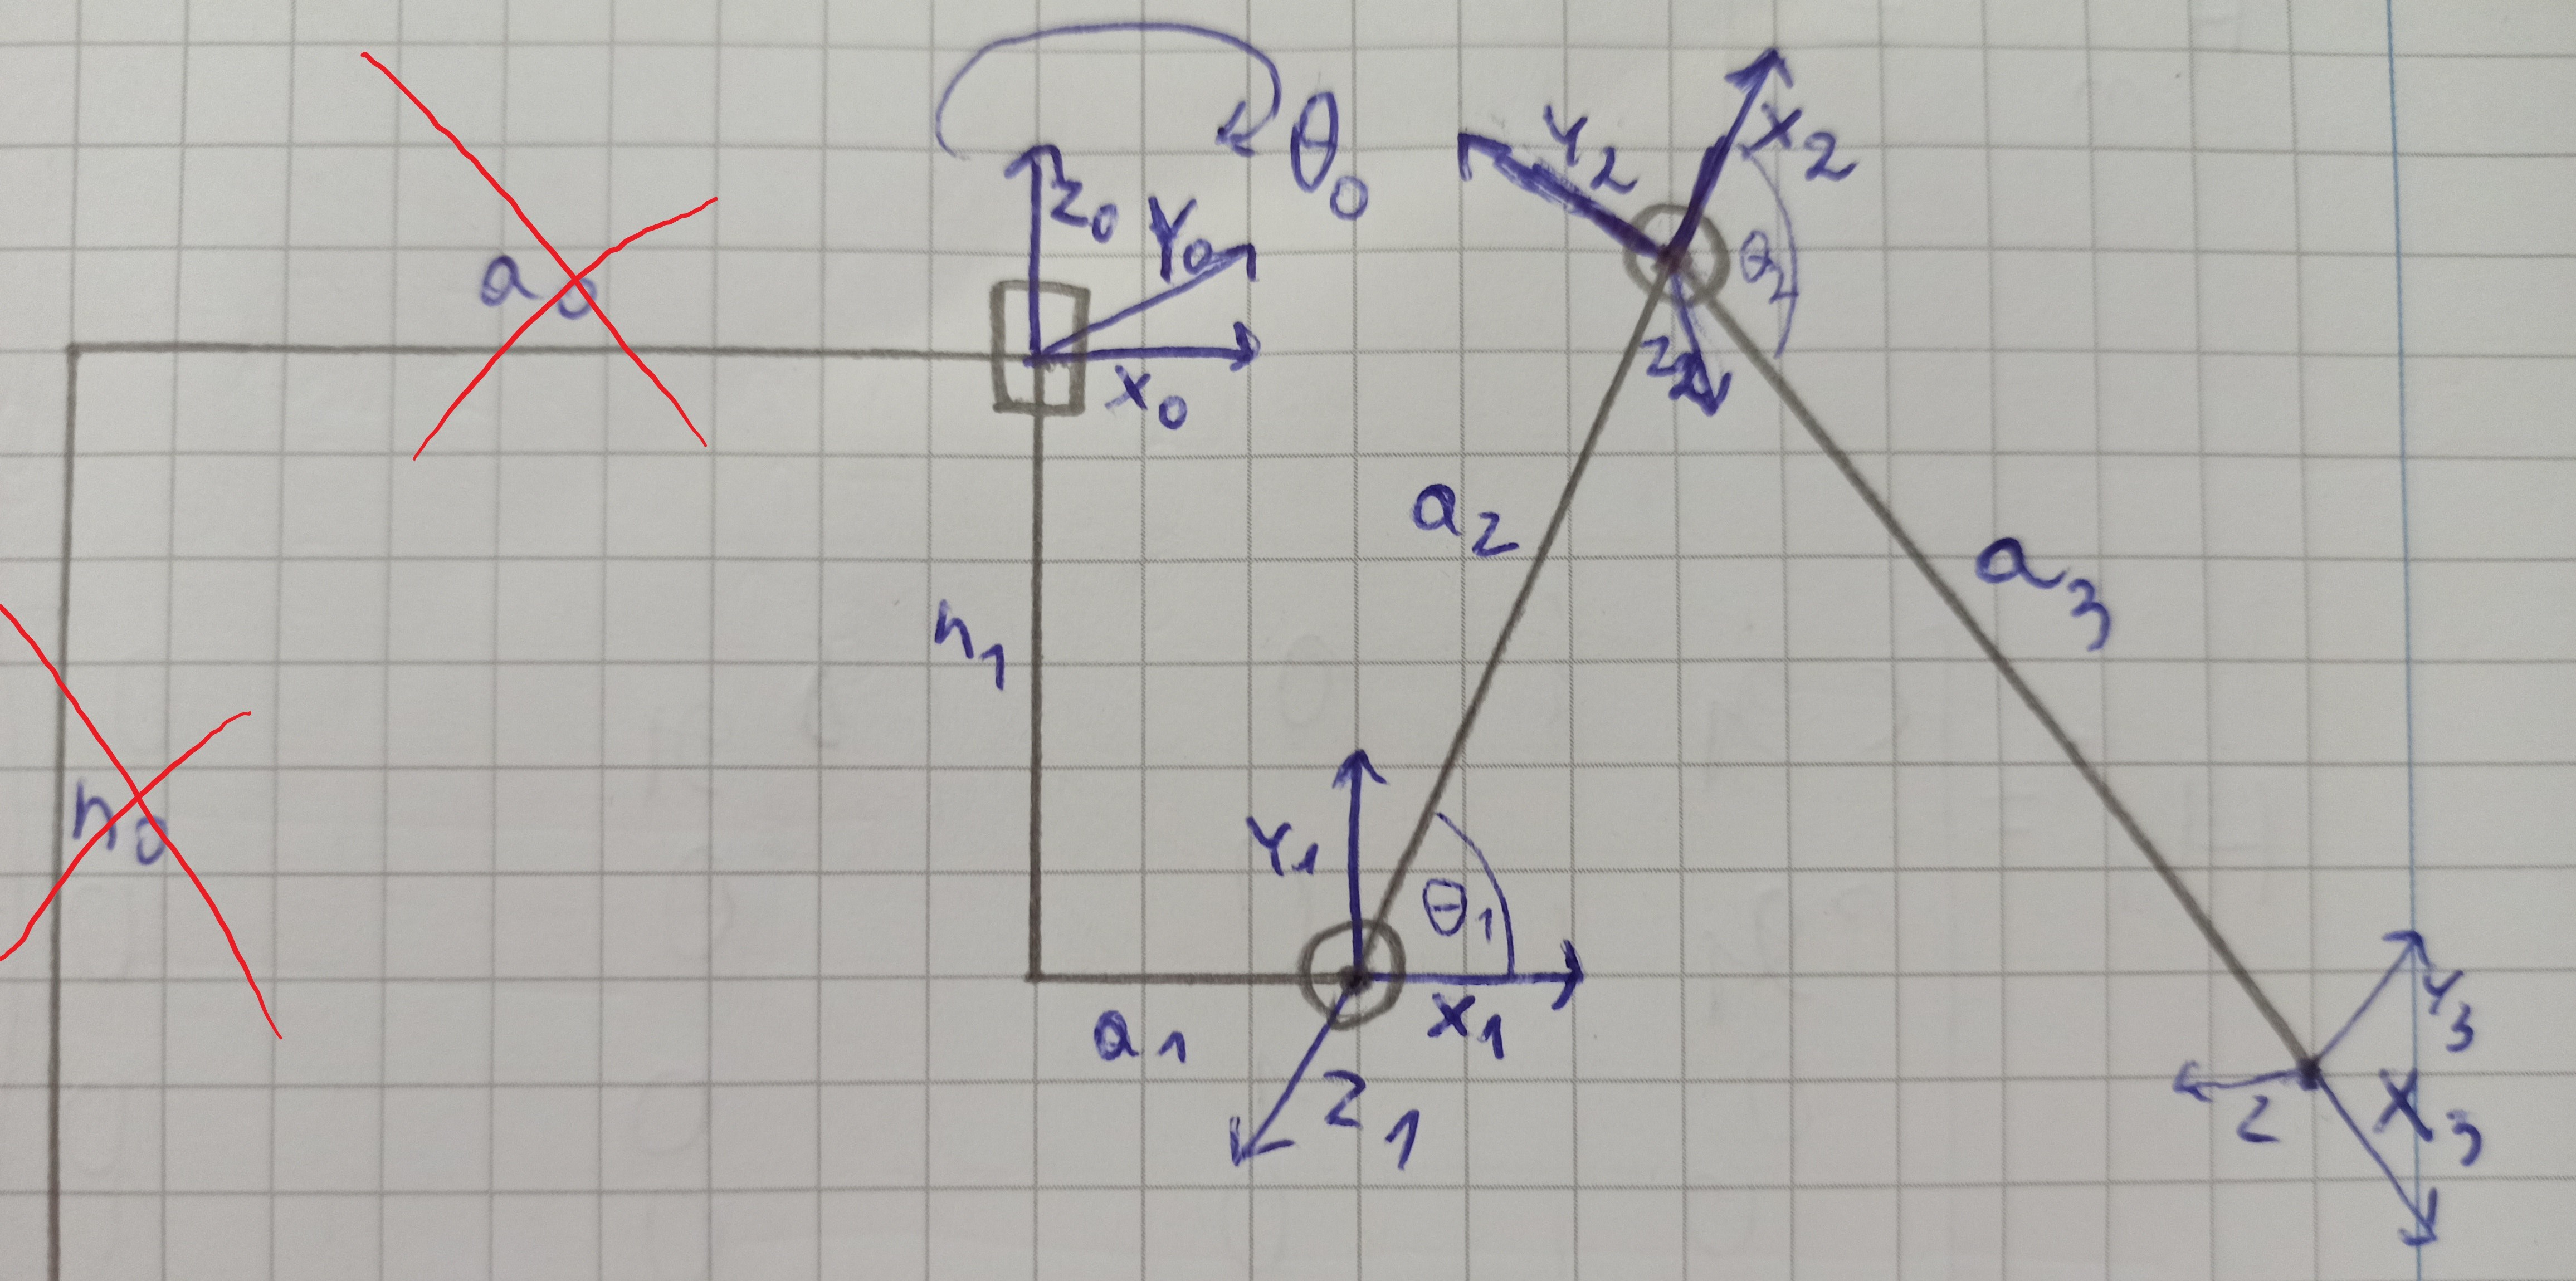
\includegraphics[width=\textwidth]{img/DH_model.jpg}
\caption{Model Denavit Hartenberg}
\label{math_model_DH}
\end{figure}

Z praktycznynego punktu widzenia obliczenia należy zacząć od stworzenia specjalnego rysunku (Rys. \ref{math_model_DH}) z zaznaczonymi kolejnymi obrotami lokalnych układów współrzędnych, a następnie zebrać odpowiednie transformacje do tabelki (Tab. \ref{table:DH_table})\\

\begin{table}[h!]
\centering
\begin{tabular}{c | c c c c }
 Joint $i$ & $\theta_i$ & $\alpha_i$ & $r_i$ & $d_i$ \\
 \hline
 $1$  & $\theta_0$ & $\frac{\pi}{2}$ & $a_1$ & $h_1$ \\
 $2$  & $\theta_1$ & $0$ & $a_2$ & $0$ \\
 $3$  & $\theta_2$ & $0$ & $a_3$ & $0$ \\
\end{tabular}
\caption{Tabela z parametrami DH}
\label{table:DH_table}
\end{table}

Gdzie: \\
$\theta_i$ - angle from $x_{n-1}$ to $x_n$ around $z_{n-1}$\\
$\alpha_i$ - angle from $z_{n-1}$ to $z_n$ around $x_n$\\
$r_i$ - distance between the origin of the $n-1$ frame and the origin of the $n$ frame along the $x_n$ direction.\\ 
$d_i$ - distance from $x_{n-1}$ to $x_n$ along the $z_{n-1}$ direction\\

Następnie macierze transformacji jednorodnej (pomiędzy ramkami $n-1$ i $n$) oblicza się zgodnie ze wzorem \ref{DH_homogenous}. Wzór ten jest właśnie obliczony poprzez wymnożenie wzorów na wyżej wspomniane 6 przekształceń prostych. Ale w zasadzie wzór ten sprowadza się do 2 zasadniczych elementów. $R$ jest macierzą Rotacji o rozmiarze $3x3$ a $T$ to macierz Transformacji $1x3$. \cite{DH_matrix_AA_article}\\

\begin{equation} \label{DH_homogenous}
H^{n-1}_n = 
\left[\begin{array}{ccc|c}
&&&\\
&&&\\
\multicolumn{3}{c|}{\smash{\raisebox{0.75\normalbaselineskip}{R}}} & \smash{\raisebox{0.75\normalbaselineskip}{T}}\\
\hline
0 & 0 & 0 & 1\\
\end{array}\right] = 
\left[\begin{matrix}
\cos{\theta_i} & -\sin{\theta_i} \cdot \cos{\alpha_i} & \sin{\theta_i} \cdot \sin{\alpha_i} & a_i \cdot \cos{\theta_i}\\
\sin{\theta_i} & \cos{\theta_i} \cdot \cos{\alpha_i} & -\cos{\theta_i} \cdot \sin{\alpha_i} & a_i \cdot \sin{\theta_i}\\
0 & \sin{\alpha_i} & \cos{\alpha_i} & d_i\\
0 & 0 & 0 & 1\\
\end{matrix}\right]
\end{equation}


Następnie należy podstawić wartości dla każdego z 3 punktów i otrzymane macierze wymnożyć zgodnie ze wzorem \ref{DH_final_equation}. Mnożenie to zostało wykonane przy pomocy skryptu napisanego w programie Matlab. %TODO - podlinkować skrypt

\begin{multline} \label{DH_final_equation}
H^{n-1}_n = H^0_1 \cdot H^1_2 \cdot H^2_3 =\\
\left[\begin{smallmatrix}
c\theta_0 \cdot \left( c\theta_1 \cdot c\theta_2 - s\theta_1 \cdot s\theta_2 \right) & -c\theta_0 \cdot \left( c\theta_1 \cdot s\theta_2 + s\theta_1 \cdot c\theta_2 \right) & s\theta_0 & c\theta_0 \cdot \left( a_1 + a_2 \cdot c\theta_1 + a_3  \cdot \left( c\theta_1 \cdot c\theta_2 - s\theta_1 \cdot s\theta_2 \right) \right)\\
s\theta_0 \cdot \left( c\theta_1 \cdot c\theta_2 - s\theta_1 \cdot s\theta_2 \right) & -s\theta_0 \cdot \left( c\theta_1 \cdot s\theta_2 + s\theta_1 \cdot c\theta_2 \right) & -c\theta_0 & s\theta_0 \cdot \left( a_1 + a_2 \cdot c\theta_1 + a_3  \cdot \left( c\theta_1 \cdot c\theta_2 - s\theta_1 \cdot s\theta_2 \right) \right)\\
c\theta_1 \cdot s\theta_2 + s\theta_1 \cdot c\theta_2 & c\theta_1 \cdot c\theta_2 - s\theta_1 \cdot s\theta_2 & 0 & h_1 + a_2 \cdot s\theta_1 + a_3 \cdot \left( c\theta_1 \cdot s\theta_2 + s\theta_1 \cdot c\theta_2 \right)\\
0 & 0 & 0 & 1\\
\end{smallmatrix}\right] = \\
\left[\begin{matrix}
c\theta_0 \cdot c\left( \theta_1 + \theta_2 \right) & -c\theta_0 \cdot s\left( \theta_1 + \theta_2 \right) & s\theta_0 & c\theta_0 \cdot \left( a_1 + a_2 \cdot c\theta_1 + a_3  \cdot c\left( \theta_1 + \theta_2 \right) \right)\\
s\theta_0 \cdot c\left( \theta_1 + \theta_2 \right) & -s\theta_0 \cdot s\left( \theta_1 + \theta_2 \right) & -c\theta_0 & s\theta_0 \cdot \left( a_1 + a_2 \cdot c\theta_1 + a_3  \cdot c\left( \theta_1 + \theta_2 \right) \right)\\
c\theta_1 \cdot s\theta_2 + s\theta_1 \cdot c\theta_2 & c\left( \theta_1 + \theta_2 \right) & 0 & h_1 + a_2 \cdot s\theta_1 + a_3 \cdot s\left( \theta_1 + \theta_2 \right)\\
0 & 0 & 0 & 1\\
\end{matrix}\right]
\end{multline}

Następnie, aby otrzymać właściwe równania, należy z równania \ref{DH_final_equation} wziąć część odpowiedzialną za transformację. Efektem jest wzór \ref{FK_ver_2_initial}, czyli finalna wersja równań kinametayki prostej obliczonej metodą Denavita Hartenberga\\

\begin{equation} \label{FK_ver_2_initial}
\begin{split}
X &= c\theta_0 \cdot \left( a_1 + a_2 \cdot c\theta_1 + a_3  \cdot c\left( \theta_1 + \theta_2 \right) \right)\\
Y &= s\theta_0 \cdot \left( a_1 + a_2 \cdot c\theta_1 + a_3  \cdot c\left( \theta_1 + \theta_2 \right) \right)\\
Z &= h_1 + a_2 \cdot s\theta_1 + a_3 \cdot s\left( \theta_1 + \theta_2 \right)\\
\end{split}
\end{equation}

Można jeszcze przetworzyć to równanie do takiej postaci w jakiej zapisane jest równanie \ref{FK_ver_1}. Otrzymamy wtedy równanie \ref{FK_ver_2}.

\begin{equation} \label{FK_ver_2}
\begin{split}
a_temp &= \left( a_1 + a_2 \cdot c\theta_1 + a_3  \cdot c\left( \theta_1 + \theta_2 \right) \right)\\
X &= \cos{\theta_0} \cdot a_temp\\
Y &= s\theta_0 \cdot a_temp\\
Z &= h_1 + a_2 \cdot s\theta_1 + a_3 \cdot s\left( \theta_1 + \theta_2 \right)\\
\end{split}
\end{equation}



TODO - znak pomiędzy obliczeniami geometrycznymi a DH się nie zgadza


\subsection{Kinematyka odwrotna}
Kinematyka odwrotna jest natomiast - jak sama nazwa wskazuje - procesem odwrotnym do kinematyki prostej. Polega na obliczeniu zestawu współrzędnych konfiguracyjnych na podstawie współrzędnych kartezjańskich końcówki manipulatora. Czyli inaczej mówiąc - wejściem algorytmu są współrzędne kartezjańskie, a wyjściem współrzędne konfiguracyjne.

Zwykle odwrotną kinematykę można obliczyć poprzez rozwiązanie równań kinematyki prostej. Jest to w tym przypadku także teoretycznie możliwe, jako że mamy do czynienia z trzema niewiadomymi ($\theta_{0-2}$) i układem trzech równań nr. \ref{FK_ver_1} (lub \ref{FK_ver_2}). (Równanie na $a_{temp}$ jest jedynie pomocnicze, trzeba je traktować jak część równań $Y$ i $X$).

Jest to jak najbardziej wykonalne w przypadku $\theta_0$, można to zrobić łącząc wzór na $X$ i $Y$, dzieląc go obustronnie, zamieniając $\frac{\sin}{\cos}$ na $\tan$ i wyciągając $\theta_0$ na lewą stronę. Daje to wzór \ref{theta_0_eq_final}

%\begin{equation}
%\begin{split}
%\begin{cases}
%Y = a_{temp} \cdot \sin{\theta_0}\\
%X = a_{temp} \cdot \cos{\theta_0}
%\end{cases}
%\end{split}
%\end{equation}

%\begin{equation}
%\begin{split}
%\begin{cases}
%Y = a_{temp} \cdot \sin{\theta_0}\\
%a_{temp} = \frac{X}{\cos{\theta_0}}
%\end{cases}
%\end{split}
%\end{equation}


%\begin{equation}
%Y = \frac{X}{\cos{\theta_0}} \cdot \sin{\theta_0}\\
%\end{equation}

\begin{equation} \label{theta_0_eq_final}
\theta_0 = \arctan{\frac{Y}{X}}
\end{equation}

%Wzór na $\theta_2$ można wyprowadzić także z równania \ref{FK_ver_1}

%\[
%Z = (- h_1) + a_2 \cdot \sin{\theta_1} - a_3 \sin{\left( \theta_2 - \theta_1 %\right)}
%\]

%\[
%z + h_1 = a_2 \cdot \sin{\theta_1} - a_3 \sin{\left( \theta_2 - \theta_1 \right)}
%\]

%\[
%\frac{h_1 - Z - a_2 \cdot \sin{\theta_1}}{a_3} = \sin{\left( \theta_2 - \theta_1 \right)}
%\]


%\begin{equation} \label{theta_2_eq}
%\theta_2 = \arcsin{\left(\frac{h_1 - Z - a_2 \cdot \sin{\theta_1}}{a_3}\right)} + \theta_1
%\end{equation}

%Równanie \ref{theta_2_eq} jest nadal uzależnione od $\theta_1$, które należy wyznaczyć.

%Najbardziej oczywistym wydaje się pod równanie \ref{FK_ver_1} na $a_{temp}$ podstawić obliczone równanie \ref{theta_2_eq} i daje to równanie  \ref{theta_1_eq1}

%\begin{equation} \label{theta_1_eq1}
%a_{temp} = a_2 \cos{\theta_1} + a_3 \cos{\left(\arcsin{\left(\frac{h_1 - Z - a_2 \cdot \sin{\theta_1}}{a_3}\right)}\right)} + a_1\\
%\end{equation}

%Do fragmentu $a_3 \cos{\left(\arcsin{\left(\frac{h_1 - Z - a_2 \cdot \sin{\theta_1}}{a_3}\right)}\right)}$ można zastosować wzór $\cos{\left(\arcsin{\left(x\right)}\right)} = \sqrt{1 - x^2}$. Daje to wzór \ref{theta_1_eq2}

%\begin{equation} \label{theta_1_eq2}
%a_{temp} = a_2 \cos{\theta_1} + \sqrt{a_3^2 - (a_2 \sin{\theta_1} - h_1 - Z)^2} + a_1\\
%\end{equation}

%Niestety wzór \ref{theta_1_eq2} nie pozwala jednoznacznie wyznaczyć jawnego $\theta_1$ i co za tym idzie nie da się tego wzoru jednoznacznie zaimplementować softwareowo, co jest niezbędne w dalszej części pracy. Można natomiast powrócić do rysunku \ref{math_model} i zastosować na trójkącie utworzonym z $a_2$ i $a_3$ twierdzenie cosinusów połączone z twierdzeniem pitagorasa.

Większy problem pojawia się jednak w przypadku obliczania $\theta_1$ i $\theta_2$, ponieważ wartości te da się obliczyć z wyżej wspomnianego równania, ale nie da się wyznaczyć na te wartości równań w postaci jawnej. A bez postaci jawnej poprawna implementacja tych równań będzie znacznie utrudniona.

Można natomiast zastosować pewnego rodzaju uproszczenie. Jeżeli wyznaczanie równań $\theta_1$ i $\theta_2$ sprowadzi się do problemu dwuwymiarowego, obliczenia stają się w zasadzie identyczne jak w przypadku obliczeń kinematyki odwrotnej dla robota typu SCARA, co było już robione wielokrotnie. \cite{SCARA_model}\\

Aby obliczyć kąt $\theta_2$ można powrócić do rysunku \ref{math_model} i zastosować na trójkącie utworzonym z $a_2$ i $a_3$ twierdzenie cosinusów połączone z twierdzeniem pitagorasa. Daje to wzór \ref{theta_2_eq_1}. \cite{SCARA_model_calc}

\begin{equation} \label{theta_2_eq_1}
(x - a_1)^2 + (z + h_1)^2 = a_2^2 + a_3^2 - 2 \cdot a_2 \cdot a_3 \cdot \cos{(180^o - \theta_2)}\\
\end{equation}

Następnie na podstawie równania \ref{theta_2_eq_1} aby ostatecznie otrzymać $\theta_2$ należy zastosować wzór $\cos{(180^o - \theta)} = -\cos{\theta}$ i za pomocą prostych przekształceń wyciągnąć z równania $\theta_2$. Daje to wzór \ref{theta_2_eq_final} \cite{SCARA_model_calc}

\begin{equation} \label{theta_2_eq_final}
\theta_2 = \arccos{\left( \frac{(x - a_1)^2 + (z + h_1)^2 - a_2^2 - a_3^2}{2 a_2 a_3} \right)}\\ 
\end{equation} 

Obliczenia dla $\theta_1$ są natomaist trochę bardziej skomplikowane. Aby dało się je prosto zwizualizować, wykonany został rysunek \ref{theta_1_model}. Na podstawie rysunku, stosując wzory trygonometryczne, można otrzymać zależności \ref{theta_1_eq_1} \cite{SCARA_model_calc}

\begin{figure}[h!]
\includegraphics[width=\textwidth]{img/theta_1_model.jpg}
\caption{Fragment modelu nogi do obliczeń $theta_1$}
\label{theta_1_model}
\end{figure}

\begin{equation}\label{theta_1_eq_1}
\begin{split}
\beta &= \arctan{\frac{a_3 \cdot \sin{\theta_2}}{a_2 + a_3 \cdot{\theta_2}}}\\
\gamma &= \arctan{\frac{-\Delta z}{\Delta x}} = - \arctan{\frac{\Delta z}{\Delta x}}\\
\theta_1 &= \gamma - \beta\\
\end{split}
\end{equation}

Do rozwiązania układu \ref{theta_1_eq_1} potrzebne są jeszcze $\Delta z$ i $\Delta x$. Na podstawie rysunku \ref{math_model} można stwierdzić że $\Delta z = Z + h_1$ a $\Delta x = X - a_1$. Podstawiając te dane pod równanie równanie 2 układu \ref{theta_1_eq_1} i podstawiając równanie 1 i 2 pod odpowiednie kąty z równania 3 wspomnianego układu otrzymujemy ostateczne rozwiązanie na $\theta_1$ - równanie \ref{theta_1_eq_final}.



\begin{equation}\label{theta_1_eq_final}
\theta_1 = \arctan{\frac{Z + h_1}{X - a_1}} + \arctan{\frac{a_3 \cdot \sin{\theta_2}}{a_2 + a_3 \cdot{\theta_2}}}\\ 
\end{equation}

Ostatecznie zbierając równania \ref{theta_0_eq_final}, \ref{theta_1_eq_final}, \ref{theta_2_eq_final} otrzymujemy układ równań \ref{inverse_eq_final} który stanowi uproszczoną kinematykę odwrotną opisywanej nogi robotycznej.

\begin{equation}\label{inverse_eq_final}
\begin{split}
\theta_0 &= \arctan{\frac{Y}{X}}\\
\theta_1 &= \arctan{\frac{Z + h_1}{X - a_1}} + \arctan{\frac{a_3 \cdot \sin{\theta_2}}{a_2 + a_3 \cdot{\theta_2}}}\\ 
\theta_2 &= \arccos{\left( \frac{(x - a_1)^2 + (z + h_1)^2 - a_2^2 - a_3^2}{2 a_2 a_3} \right)}\\
\end{split}
\end{equation}

TODO - ograniczenia.

Natomiast trzeba cały czas pamiętać że jest to tylko uproszczenie, które będzie owocować pewnymi drobnymi błędami. Trzeba zauważyć, że zmiana współrzędnej $Y$ nie wpływa na wartości kątów $\theta_1$ i $\theta_2$, tylko na $\theta_0$. Oznacza to, że wraz ze zmianą kąta $\theta_0$, na potrzeby uproszczenia obliczeń, obraca się także o ten kąt oś $X$ układu współrzędnych. W praktyce oznacza to, że odsunięcie nogi od punktu $(0, 0, 0)$ zawsze będzie rzutowane na cylinder o promieniu równym odsunięciu o takim samym $X$ i $Z$, ale $Y = 0$. Problem jest zaprezentowany na rysunku \ref{SCARA_error}. Na obrazku tym widać pozycję początkową robota oznaczoną jako "0". Następnie jeśli robot wykona krok, to stosując ten algorytm, znajdzie się w pozycji "1p", a w idealnym przypadku powinien znaleźć się w "1i". Jednakże błąd powinien być pomijalnie mały a równania powinny umożliwić skuteczną implementację algorytmu chodu.

\begin{figure}[h!]
\includegraphics[width=\textwidth]{img/SCARA_error.jpg}
\caption{Przedstawienie błędu spowodowanego zastosowaniem modelu robota SCARA przy kinematyce odwrotnej}
\label{SCARA_error}
\end{figure}


\section{Cały Robot}
Zwykle konstruując roboty wzorujemy się na zwierzętach występujących w naturze. W tym przypadku nie mamy jednak tego luksusu, dlatego na początek należy przyjąć jakieś najbardziej intuicyjne założenie. Dlatego też uznałem że najlepszym rozwiązaniem będzie rozmieścić nogi na jednej płaszczyźnie w równych odstępach - co $120\deg$.

W poprzednim podrozdziale przyjąłem osie układu relatywne do ułożenia początkowego nogi robota. Oznacza to że robot trójnożny będzie miał 3 niezależne osie $x$ i 3 niezależne osie $y$, tylko oś $z$ zgadza się między kolejnymi nogami. Idzie za tym konieczność stworzenia pewnej metody "obracania" wszystkich tych osi $x$ i $y$ do jednego zunifikowanego układu współrzędnych. Pozwoli to obliczyć kinematykę całego robota.

\subsection{Matematyka kroku}
W celu uproszczenia zarówno obliczeń jak i późniejszej generacji kolejnych kroków algorytmu chodu, można pominąć liczenie całej kinematyki prostej i odwrotnej całego robota. Zamiast tego wystarczy pojedynczy krok odpowiednio sparametryzować. Jeżeli dla każdego kroku pojedynczej nogi przyjmiemy:
\begin{itemize}[noitemsep]
\item kąta $\alpha$ na "tarczy" robota, na którym ustawiona jest noga
\item kąta $\beta$ względem "przodu" robota, w którą ma zostać wykonany krok
\item długość kroku $l$, równolegle do osi kroku robota
\end{itemize}
To możemy łatwo otrzymać algorytm który z tych dwóch zmiennych i jednej stałej da pozycję zmianę pozycji końcówki robota ($\Delta x, \Delta y$) we współrzędnych kartezjańskich względem nogi robota.

\begin{figure}[h!]
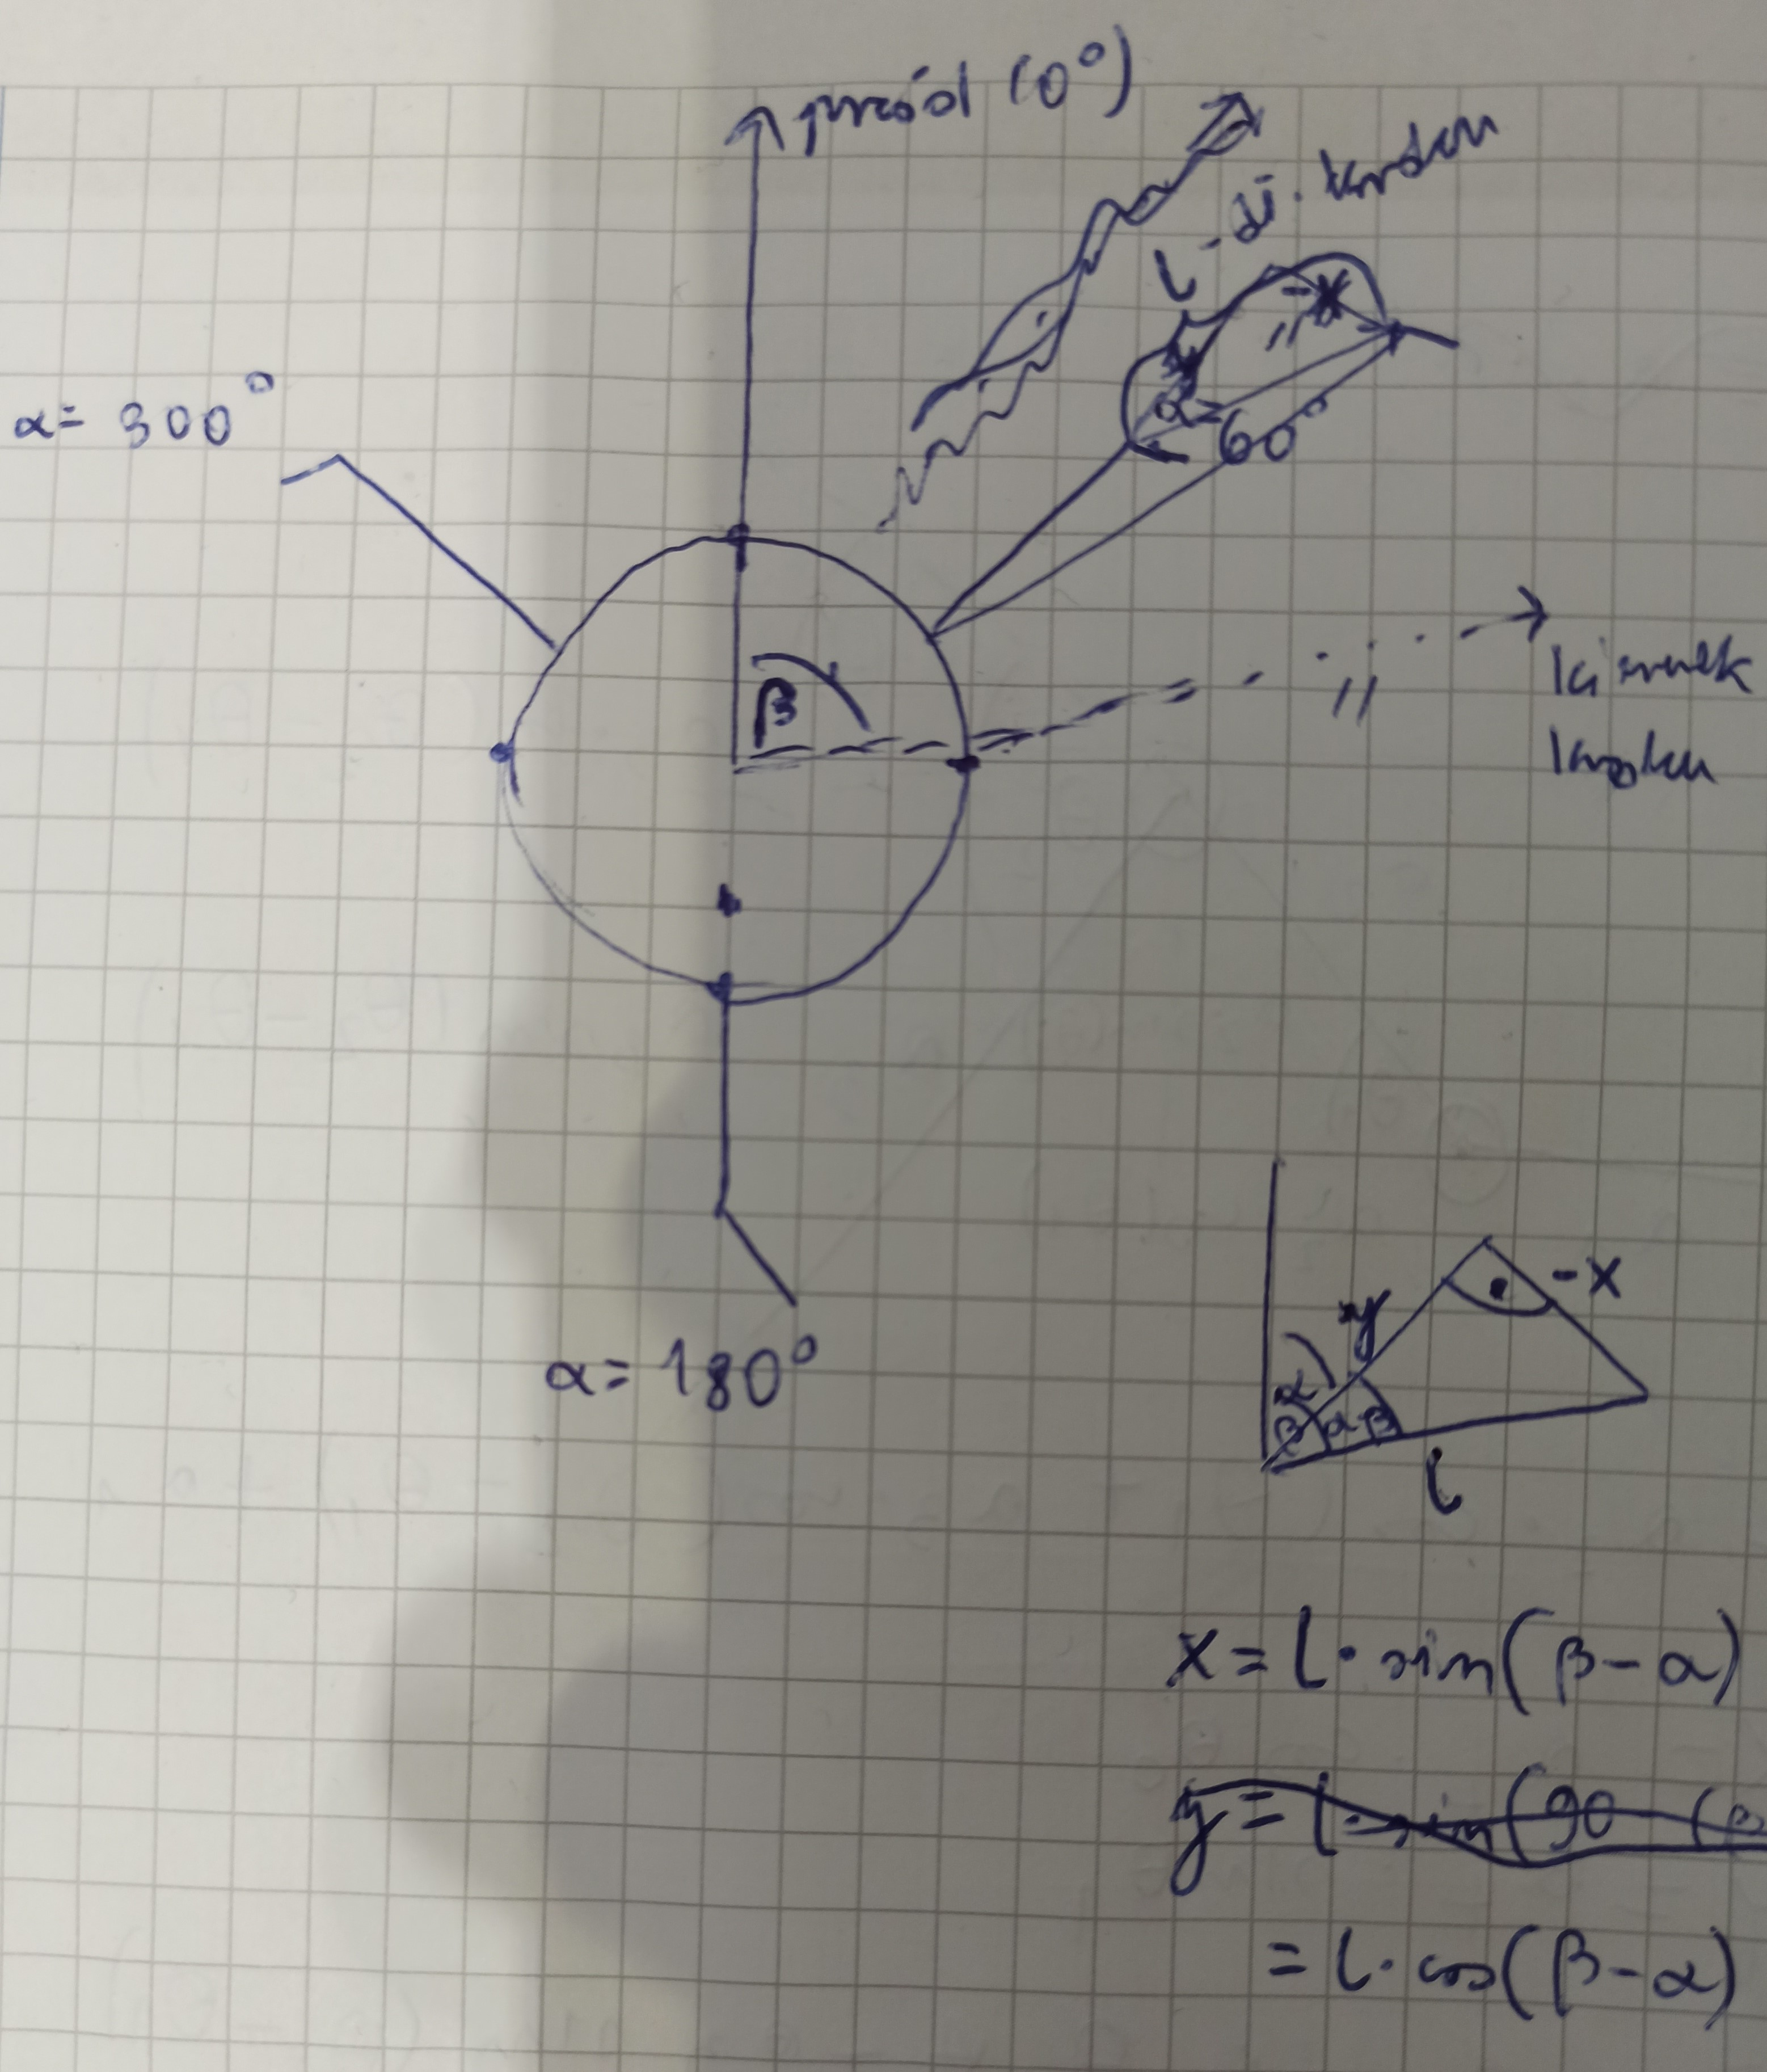
\includegraphics[width=\textwidth]{img/step_math.jpg}
\caption{Schemat matematyczny wykonywania kroku}
\label{step_math}
\end{figure}

Zostało to przedstawione na rysunku \ref{step_math} na przykładzie nogi na pozycji $\alpha = 60^o$. Na wspomnianym rysunku widać przód robota oznaczony jako $0^o$, kierunek kroku odsunięty o kąt $\beta$ od osi "przodu" robota i wynikające z tego kroku przestawienie nogi. Przestawienie to składa się z długości korku $l$ i dwóch pozycji nogi - przed krokiem i po kroku. Wynikające z tego zależności geometryczne zostały wyizolowane na rysunku \ref{step_math_isolated}. Na podstawie tych zależności można napisać równanie \ref{step_math_eq}

\begin{figure}[h!]
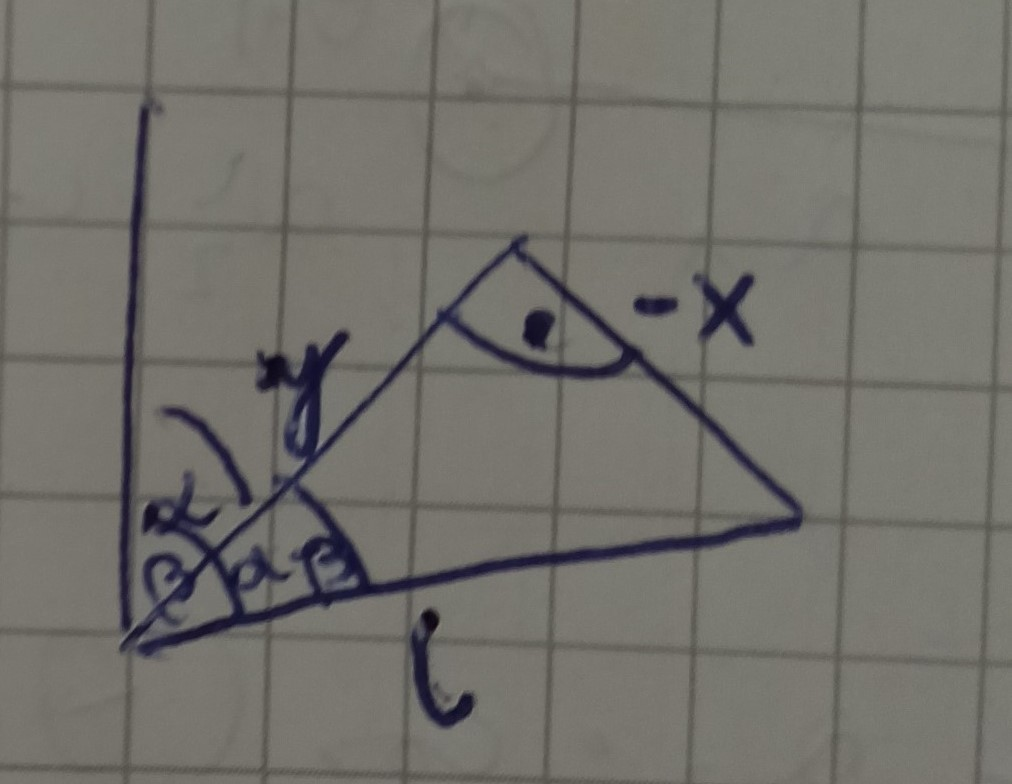
\includegraphics[width=\textwidth]{img/step_math_isolated.jpg}
\caption{Wyizolowane zależności geometryczne w czasie wykonywania kroku}
\label{step_math_isolated}
\end{figure}



\begin{equation} \label{step_math_eq}
\begin{split}
\Delta x = l \cdot \sin(\beta - \alpha)\\
\Delta y = l \cdot \cos(\beta - \alpha)\\
\end{split}
\end{equation}

Równanie \ref{step_math_eq} mówi tyle, że wykonanie nogą na pozycji $\alpha$ kroku o długości $l$ w kierunku $\beta$ wymusza przestawienie końcówki nogi o ($\Delta x$, $\Delta y$)


